%!TEX root = ../main.tex

\section{Introduction}
\label{sec:introduction}

% Close look at wall
\begin{figure}[t]
  \centering
  % \includegraphics[height=0.55\columnwidth, width=\columnwidth]{2d_delaunay.png}
  % \vspace{0.1em}
  % \includegraphics[height=0.55\columnwidth, width=\columnwidth]{spr_overview.png}
  % \includegraphics[trim={5cm 20cm 20cm 0},clip,width=0.506\columnwidth]{wall_no_smooth.png}
  % \hspace{-1.0em}
  % \includegraphics[trim={5cm 20cm 20cm 0},clip,width=0.506\columnwidth]{wall_smooth.png}
  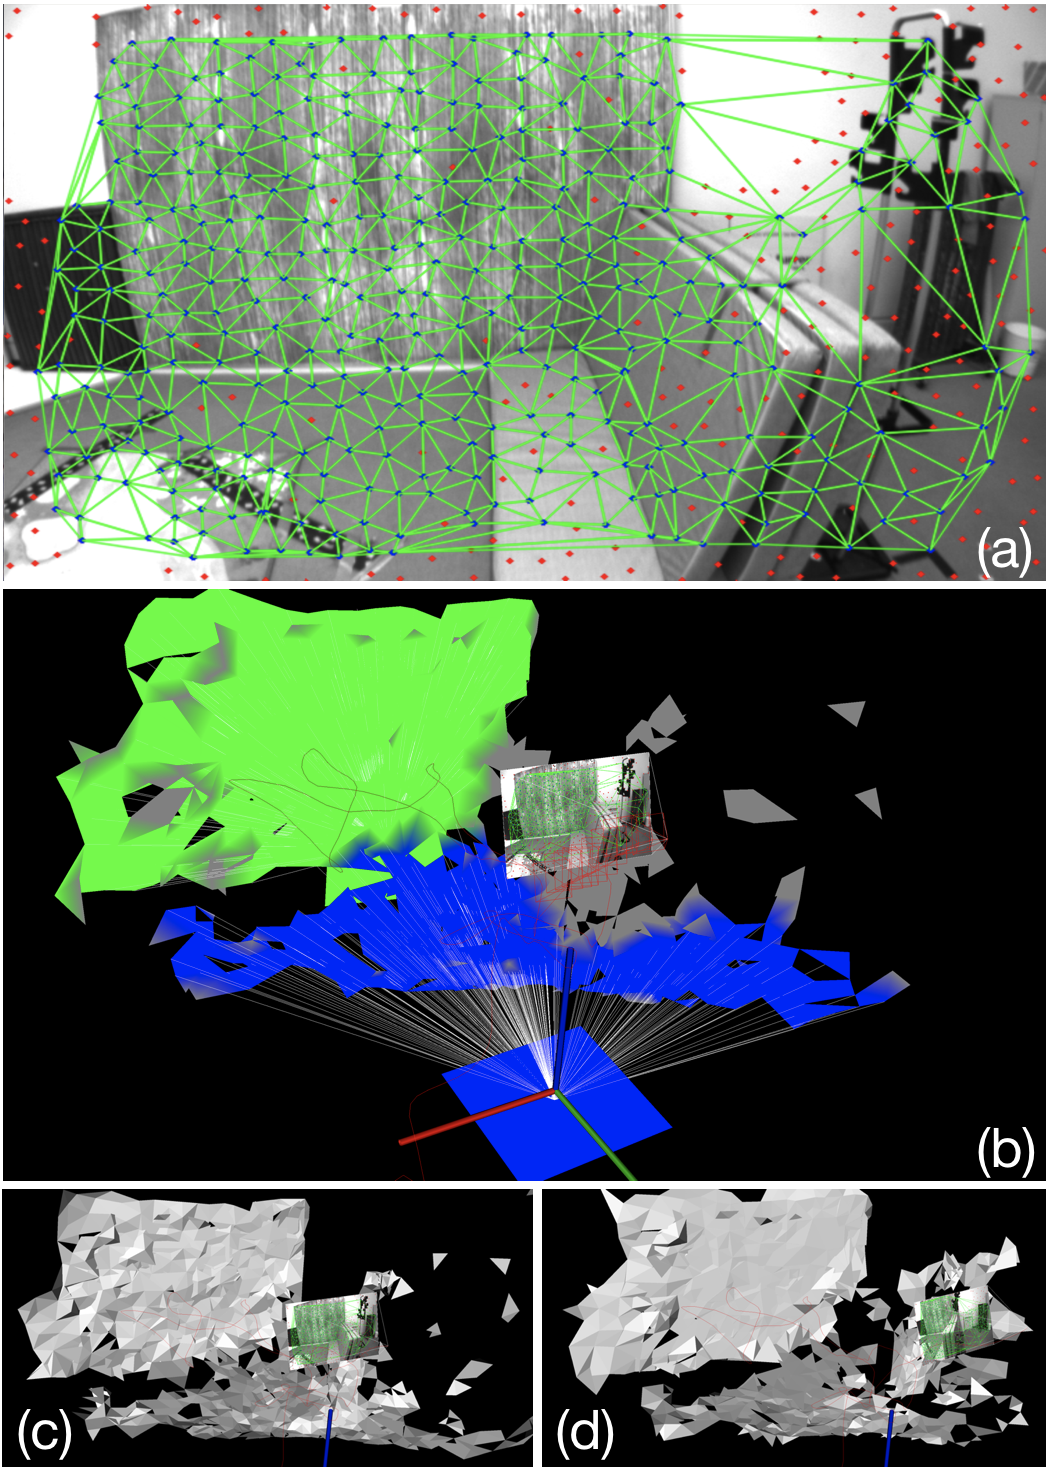
\includegraphics[width=\columnwidth]{overview4.png}
  %\subcaption{Mesh estimate without enforcing co-planarity constraints.}
  %\subcaption{Mesh estimate when enforcing co-planarity constraints.}
  \caption{We propose a VIO pipeline that incrementally builds a 3D mesh of the environment starting from (a) a 2D Delaunay triangulation of keypoints. We also detect and enforce \emph{structural regularities}, c.f.~(b) planar walls (green) and floor (blue). The bottom row in the figure compares the mesh constructed
  (c) without and (d) with structural regularities.\vspace{-5mm}}
  %Subfigures (c) and (d) show the mesh model  }
  %Visual comparison of the mesh with (bottom) and without (top) co-planarity constraints enforced.}
  \label{fig:intro}
\end{figure}

% Drop letter for first word of the Introduction
% Use only for final version.
% In recent years, great progress has been achieved using visual and inertial information (\cite{Mourikis07icra,Leutenegger15ijrr,Forster17troOnmanifold}).
% Unfortunately, these systems have nowadays two limitations that we want to address in this work, and which we detail below.
 \IEEEPARstart{R}{ecent} advances in VIO are enabling a wide range of applications, ranging from
 virtual and augmented reality to agile drone navigation~\cite{SayreMcCord18icra}.
 %Those applications are characterized by the need for low-latency estimates to be computed on computationally-constrained platforms, hence they demand for lightweight algorithms and implementations.

{\bf Contributions.}
In this paper, we propose to \emph{incrementally build a 3D mesh restricted to the receding horizon of the VIO optimization.}
In this way, we can map larger areas than a per-frame approach, while memory footprint and computational complexity associated to the mesh remain bounded.

{\bf Paper Structure.}
Section~\ref{sec:mathematical_formulation} presents the mathematical formulation of our approach, and discusses the implementation of %both %discussing both % the structure of our
our VIO front-end and back-end. % of our VIO.
Section~\ref{sec:results} reports and discusses the experimental results and comparison against related work. Section~\ref{sec:conclusions} concludes the paper.